\documentclass{article}
\usepackage[utf8]{inputenc}
\usepackage{titling}
\usepackage{graphicx}
\usepackage{xcolor}
\usepackage[colorlinks=true,linkcolor=darkgray]{hyperref}
\usepackage[spanish]{babel}


\title{Servidor de Correo}
\author{Cristina Díaz García}
\date{Febrero 2019}

\renewcommand\maketitlehooka{\null\mbox{}\vfill}
\renewcommand\maketitlehookd{\vfill\null}


\begin{document}

\addcontentsline{toc}{section}{Índice general}

\begin{titlingpage}
\maketitle
\end{titlingpage}

\newpage

\tableofcontents

\newpage

\section{Preliminares}

\subsection{Configuración de red estática}

\begin{center}
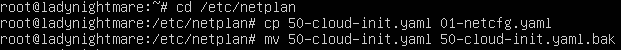
\includegraphics[scale=0.6]{images/estatica.png}
\end{center}

Modificamos el archivo .yaml para asignarle la IP estática:

\begin{center}
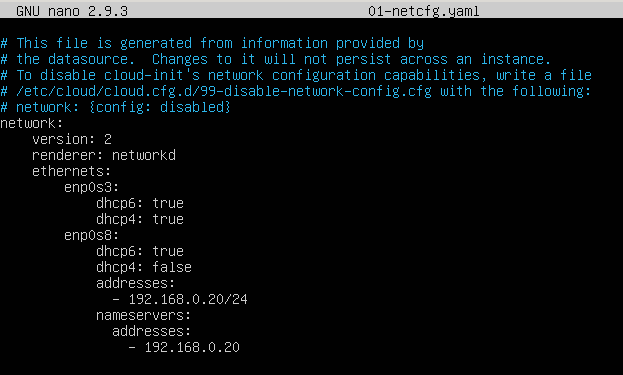
\includegraphics[scale=0.6]{images/yaml.png}
\end{center}

Tenemos dos redes configuradas, es por eso que aparecen tanto \textit{enp0s3} como \textit{enp0s8}.

\subsection{Instalación de Apache y PHP}

\begin{center}
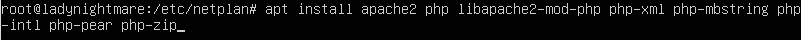
\includegraphics[scale=0.5]{images/apachePHP.png}
\end{center}

\subsection{Instalación de zip/unzip, Git y composer}

\begin{center}
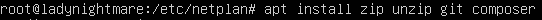
\includegraphics[scale=0.6]{images/zipunzipgitcomposer.png}
\end{center}

\subsection{Servidor Apache, Bind9 y zona directa/inversa}

\begin{center}
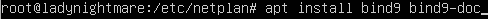
\includegraphics[scale=0.6]{images/bind9.png}
\end{center}

\begin{center}
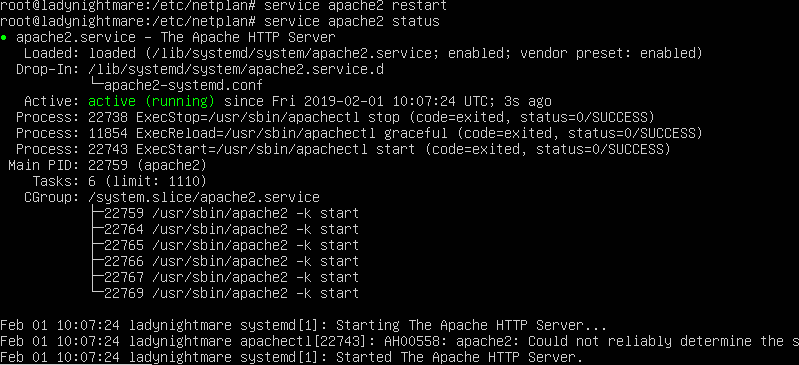
\includegraphics[scale=0.4]{images/apacheRestart.png}
\end{center}

Escribimos en el archivo de configuración de bind nuestras zonas directa e inversa.

\begin{center}
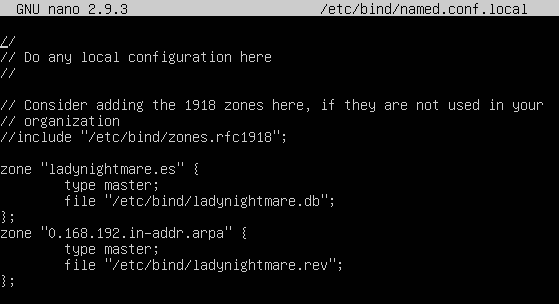
\includegraphics[scale=0.6]{images/zone.png}
\end{center}

Creamos el fichero de zona directa y lo editamos.

\begin{center}
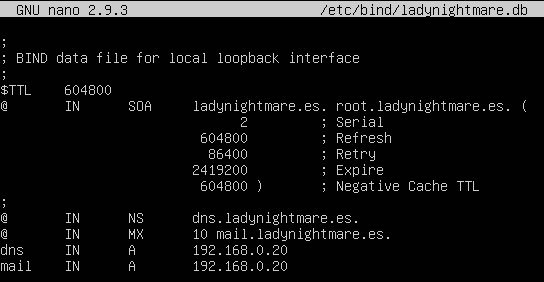
\includegraphics[scale=0.5]{images/directa.png}
\end{center}

Hacemos lo mismo con la zona inversa.

\begin{center}
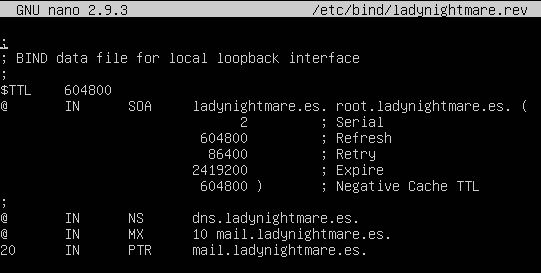
\includegraphics[scale=0.6]{images/inversa.png}
\end{center}

\subsection{Modificación de \textit{/etc/php/7.2/apache2/php.ini}}

Añadimos las extensiones necesarias:

\begin{center}
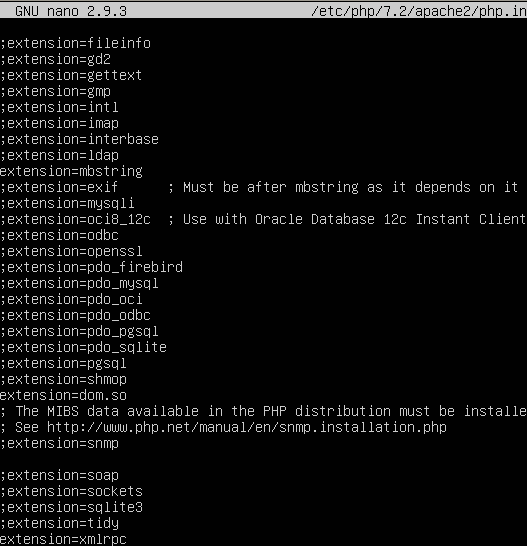
\includegraphics[scale=0.6]{images/extensiones.png}
\end{center}

También configuramos el huso horario y el tamaño máximo de los archivos.

\begin{center}
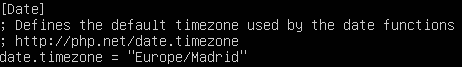
\includegraphics[scale=0.6]{images/timezone.png}
\end{center}

\begin{center}
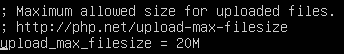
\includegraphics[scale=0.6]{images/filesize.png}
\end{center}

\begin{center}
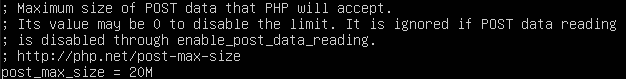
\includegraphics[scale=0.6]{images/postSize.png}
\end{center}

\begin{center}
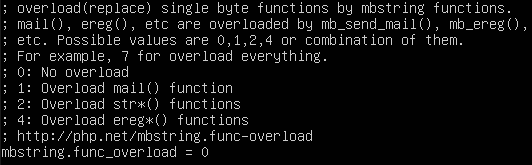
\includegraphics[scale=0.6]{images/funcOverload.png}
\end{center}

\subsection{Comprobamos los ficheros de zona}

\begin{center}
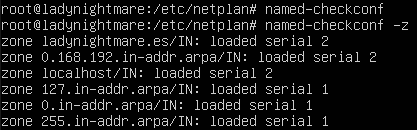
\includegraphics[scale=0.6]{images/check.png}
\end{center}

\subsection{Reiniciamos Bind y añadimos las reglas}

\begin{center}
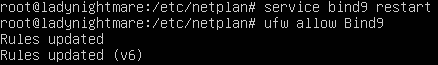
\includegraphics[scale=0.6]{images/reinicioReglas.png}
\end{center}

\subsection{MySQL}

Instalamos MySQL:

\begin{center}
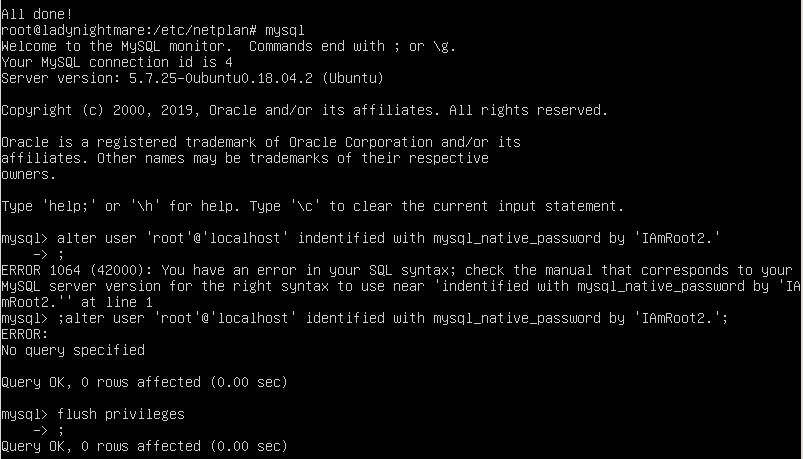
\includegraphics[scale=0.4]{images/mysql.png}
\end{center}

\subsection{Postfix}

Instalamos Postfix:

\begin{center}
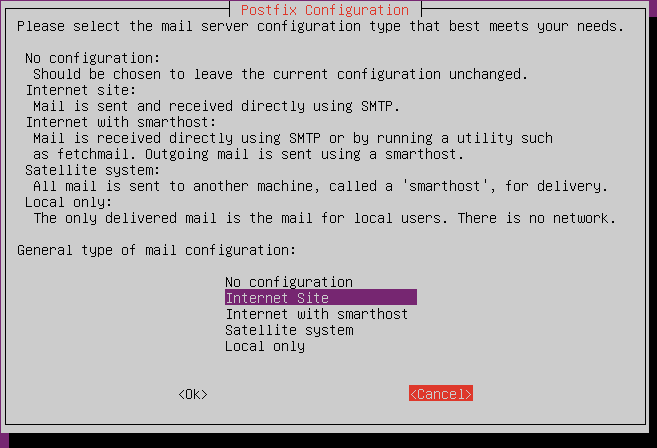
\includegraphics[scale=0.6]{images/postfix.png}
\end{center}

Y reiniciamos el servicio:

\begin{center}
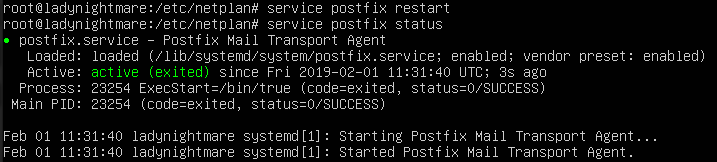
\includegraphics[scale=0.6]{images/postfixR.png}
\end{center}

Creamos el directorio donde se guardarán los correos y las tablas de mapeo de correo y las cuentas del sistema:

\begin{center}
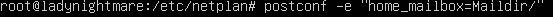
\includegraphics[scale=0.6]{images/homemailbox.png}
\end{center}

\begin{center}
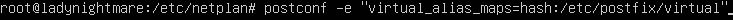
\includegraphics[scale=0.6]{images/hash.png}
\end{center}

\begin{center}
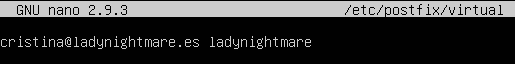
\includegraphics[scale=0.6]{images/virtual.png}
\end{center}

\begin{center}
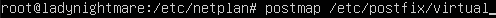
\includegraphics[scale=0.6]{images/postmap.png}
\end{center}

Reiniciamos Postfix y añadimos las reglas al firewall:

\begin{center}
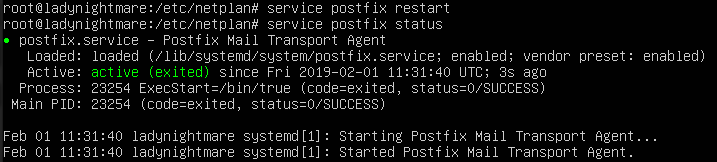
\includegraphics[scale=0.6]{images/postfixR.png}
\end{center}

\subsection{S\-nail}

\begin{center}
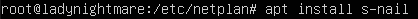
\includegraphics[scale=0.6]{images/snail.png}
\end{center}

Configuramos que se pueda enviar un correo sin tener el árbol de directorios y que se guarde una copia de los mensajes enviados.

\begin{center}
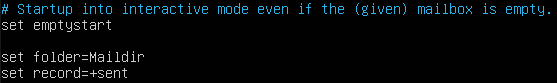
\includegraphics[scale=0.6]{images/emptystart.png}
\end{center}

Añadimos una variable de entorno MAIL para usarlo en cada inicio de sesión:

\begin{center}
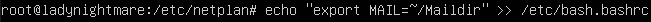
\includegraphics[scale=0.6]{images/bash.png}
\end{center}

\begin{center}
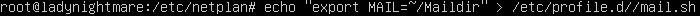
\includegraphics[scale=0.6]{images/export.png}
\end{center}

\begin{center}
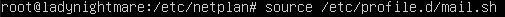
\includegraphics[scale=0.6]{images/source.png}
\end{center}

\section{Enviamos correos}

\subsection{Creamos los usuarios}

Creamos los usuarios zipi y zape:

\begin{center}
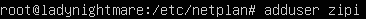
\includegraphics[scale=0.6]{images/zipi.png}
\end{center}

\begin{center}
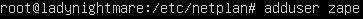
\includegraphics[scale=0.6]{images/zape.png}
\end{center}

Mandamos un correo a zipi:

\begin{center}
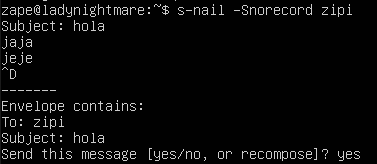
\includegraphics[scale=0.6]{images/correo.png}
\end{center}

\begin{center}
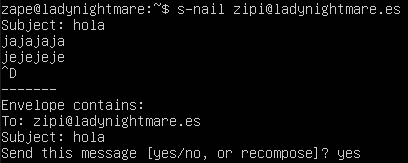
\includegraphics[scale=0.6]{images/mail.png}
\end{center}

Nos autenticamos en los usuarios y comprobamos que los directorios están creados:

\begin{center}
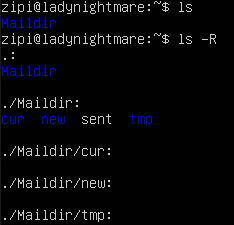
\includegraphics[scale=0.6]{images/dir.png}
\end{center}

Comprobamos los correos:

\begin{center}
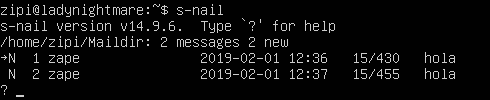
\includegraphics[scale=0.6]{images/correos.png}
\end{center}

\subsection{Courier}

Instalamos el paquete de courier:

\begin{center}
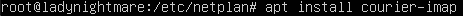
\includegraphics[scale=0.6]{images/courier.png}
\end{center}

\subsection{Roundcube}

Nos descargamos Roundcube del repositorio de GitHub y lo descomprimimos:

\begin{center}
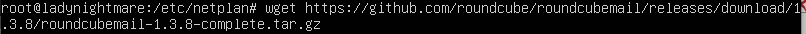
\includegraphics[scale=0.6]{images/roundcube.png}
\end{center}

\begin{center}
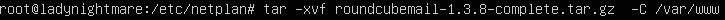
\includegraphics[scale=0.6]{images/tar.png}
\end{center}

Cambiamos los permisos y el propietario:

\begin{center}
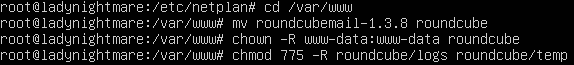
\includegraphics[scale=0.6]{images/perm.png}
\end{center}

Cambiamos la configuración:

\begin{center}
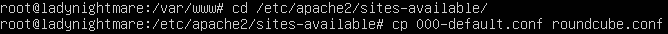
\includegraphics[scale=0.6]{images/conf.png}
\end{center}

\begin{center}
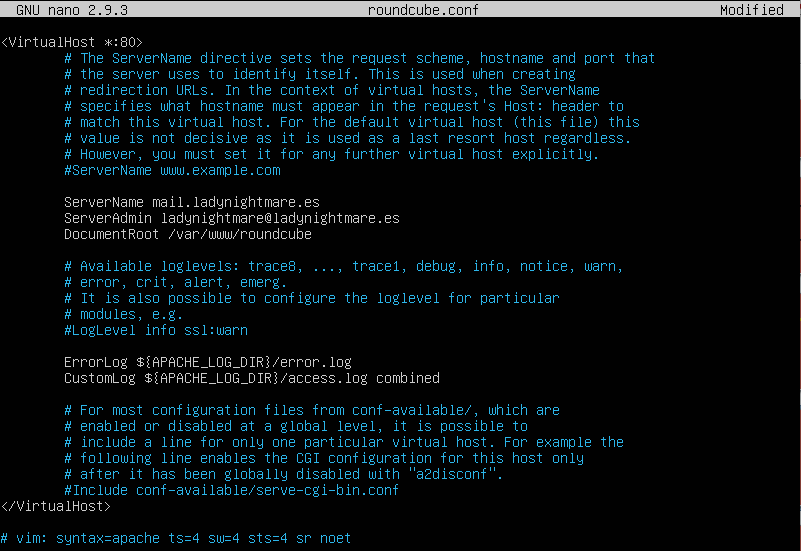
\includegraphics[scale=0.4]{images/rconf.png}
\end{center}

\begin{center}
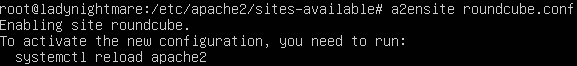
\includegraphics[scale=0.6]{images/en.png}
\end{center}

\begin{center}
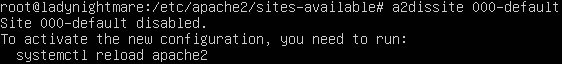
\includegraphics[scale=0.6]{images/dis.png}
\end{center}

\begin{center}
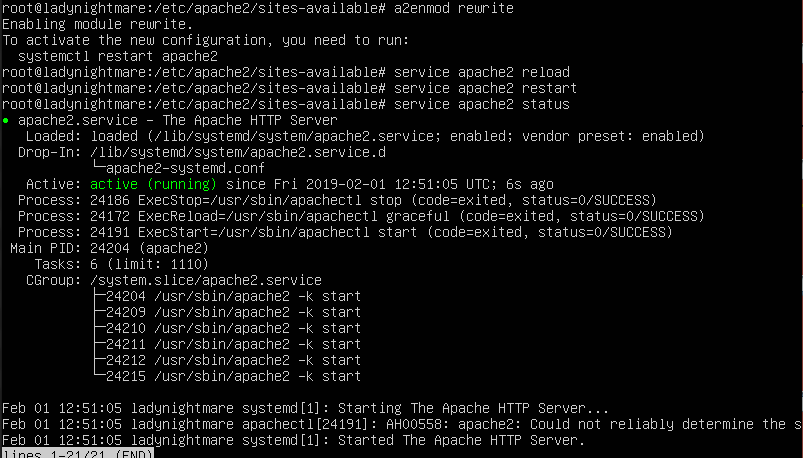
\includegraphics[scale=0.4]{images/status2.png}
\end{center}

Creamos una tabla y un usario:

\begin{center}
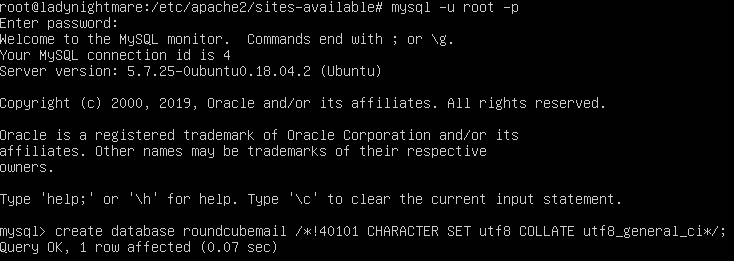
\includegraphics[scale=0.6]{images/query.png}
\end{center}

\begin{center}
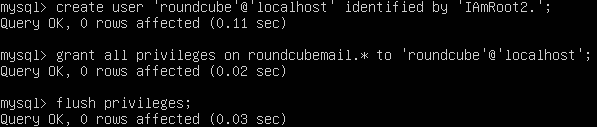
\includegraphics[scale=0.6]{images/priv.png}
\end{center}

Cargamos la información en la base de datos:

\begin{center}
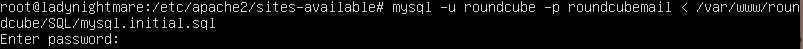
\includegraphics[scale=0.4]{images/info.png}
\end{center}

Accedemos a \textit{http://mail.ladynightmare.es/installer}:

\begin{center}
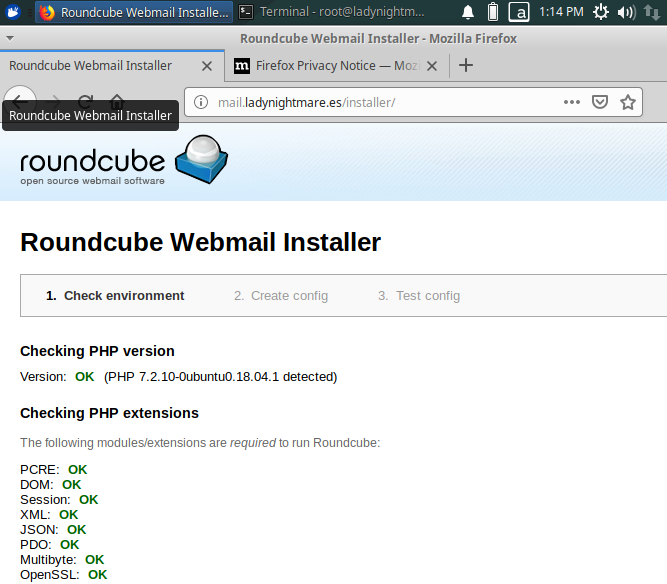
\includegraphics[scale=0.6]{images/webmail.png}
\end{center}

\begin{center}
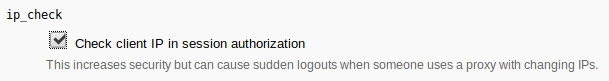
\includegraphics[scale=0.6]{images/ipcheck.png}
\end{center}

\begin{center}
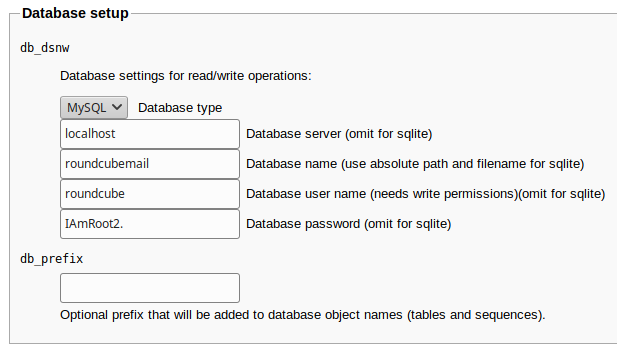
\includegraphics[scale=0.6]{images/db.png}
\end{center}

Accedemos al correo y comprobamos que, efectivamente, podemos ver nuestra bandeja de entrada.

\begin{center}
\includegraphics[scale=0.4]{images/final.png}
\end{center}

\begin{center}
\includegraphics[scale=0.4]{images/login.png}
\end{center}

\begin{center}
\includegraphics[scale=0.4]{images/last.png}
\end{center}

\end{document}
